\documentclass{scrartcl}
\usepackage{german}
\usepackage[utf8]{inputenc}
\usepackage[german]{babel}
\usepackage{amssymb}  % advanced mathematical symbold
\usepackage{graphicx} % using graphics
\usepackage{fancyhdr} % for the head of the page
\usepackage{lastpage} % makes page numbers work
\setlength{\parskip}{\medskipamount} % thats reasonable
\setlength{\parindent}{0pt}

\usepackage{wrapfig}


%%%%%%%%%%%%%%%%%%%%%%%%
% Kopf- und Fusszeilen %
%%%%%%%%%%%%%%%%%%%%%%%%
\pagestyle{fancy}
\lhead{
    \begin{tabular}{ll}
        Felix Karg & 4342014\\
    \end{tabular}
}
\chead{Superturingmaschinen}
\rhead{
    \begin{tabular}{rr}
        \today{} \\
        Seite \thepage{} von \pageref{LastPage}
    \end{tabular}
}
\lfoot{}
\cfoot{}
\rfoot{}

\title{Superturingmaschinen}
\author{Felix Karg}

%%%%%%%%%%%%%%%%%%%%%%%%
% Anfang des Dokuments %
%%%%%%%%%%%%%%%%%%%%%%%%
\begin{document}
\maketitle

\textbf{\large {Abstract:} } \\
Superturingmaschinen sind eigentlich nur Turingmaschinen, die wir nach dem Ende
der Zeit betrachten können, wodurch wir also z.B. das Klassische Halteproblem
lösen. Turingmaschinen sind ein Klassisches Beispiel für Hypercomputation, also
eine Berechenbarkeitsstufe über traditionellen Turingmaschinen, die allerdings
Physisch fragwürdig realistisch umzusetzen ist. Dennoch ergeben sich ein paar
interessante Eigenschaften, die genauer beleuchtet werden sollen.


\section{Berechenbarkeit}
Es gibt (wie allgemein bekannt ist) verschiedene Stufen der Berechenbarkeit,
wobei die einfachste Kombinatorische Logik (einfache, nicht-Zyklische
Schaltkreise) ist, und weitergehende über $DEA$ (Determistische Endliche
Automaten), $PDA$ (Push-Down-Automaton, dt: Kellerautomaten)
bis hin zu Turingmaschinen, die schon bereits alles Berechenbare berechnen
können. Häufig wird also z.B. eine Programmiersprache daran gemessen, ob sie
Turingvollständig ist, ob also alle Berechenbaren Funktionen berechnet werden
können. Neben Turingmaschinen gibt es (in den für realistische berechenbarkeit
betrachteten Bereichen) auch andere Modelle der Berechenbarkeit, z.B.
Registermaschinen, Generell-Rekursive Funktionen oder das Lambda-Kalkül.


\subsection{Konstrukt Turingmaschine}
Eine Turingmaschine ist eigentlich eine einfache, konzeptionell aber
robuste Konstruktion. Ich werde gleich noch näher darauf eingehen dass es
verschiedene, aber im Endeffekt äquivalente, Turingmaschinen gibt. (hier keine
formale Definition, da es nicht Hauptteil des Vortrages ist sowie wenig
hilfreich für das Verständnis). \\
Im Kern besteht eine Turingmaschine aus folgenden Elementen: Ein Band, das
ein Anfang hat aber nach rechts hin unendlich lange ist, also kein Ende hat.
Die eigentliche Maschine besteht aus einem kombinierten Lese- und Schreibkopf,
welcher auf dem Band operiert. Neben dem Initialzustand hat sie lediglich eine
endliche Menge an Zuständen. \\
Pro 'Berechnungsschritt'
passiert nun folgendes: Die Turingmaschine liest ein Zeichen vom Band und
entscheidet in Abhängigkeit ihres momentanen Zustandes was sie als nächstes tut.
Möglich sind: Das aktuelle Zeichen so belassen, es überschreiben, das Band nach
rechts oder links bewegen, sowie entsprechend der Übergangsfunktion eventuell
den Zustand wechseln.


\subsection{Eigenschafen von Turingmaschinen}
Relevant für uns ist im Folgenden, dass es gewisse Definitionen beziehungsweise
Arten von Turingmaschinen gibt, die der vorgestellten Äquivalent sind. Ein
% Geht es hier um genau eine Turingmaschine, die alle nachfolgenden
% Eigenschaften hat, oder geht es um mehrere? -> Entsprechend Ein Beispiel zu
% Beispiele dafuer anpassen.
Beispiel wäre eine Turingmaschine die auf zwei oder mehr Bändern rechnet
(die beide unendlich lang sind), eine die auf einem Band rechnet das in beide
Seiten unendlich lang ist, eine die in ihrem Alphabet nur $\{0, 1\}$ hat sowie
eine die ein beliebig langes, endliches Alphabet zur verfügung hat. Eine sehr
interessante Eigenschaft ist, dass unsere Turingmaschine mit ihren endlich
vielen Zuständen eindeutig definiert ist, Sie also auch entsprechend Codiert
werden kann und von einer anderen gelesen und simuliert werden kann. Daraus
ergibt sich auch dass eine Turingmaschine gleichzeitig mehrere simulieren kann,
% Mir ist hier nicht ganz klar, wovon sie mehrere simulieren kann - mehrere
% Turingmaschinen?
wofür man nun einfacherhalber gerne eine mit mehreren Bändern verwendet, um die
simulierten Turingmaschinen seperat zu halten und genauer betrachten zu können. \\
Außerdem gibt es das Halteproblem, also dass bereits bei einer Turingmaschine
mit sehr wenigen Zuständen kein Zuverlässiger Algorithmus existieren kann, der
entscheidet ob diese irgendwann hält (Terminiert, ein Ergebnis liefert) oder
eben nicht.


\subsection{Aussagentypen}
Eine Teilmenge $M \subseteq \mathbb{N}$ ist genau dann von einer Turingmaschine
aufzählbar (oder rekursiv aufzählbar) sofern es eine Turingmaschine gibt, die
in beliebiger Reihenfolge alle Elemente dieser Menge auf das Band schreiben
kann. Eine solche Menge wird $\Sigma_1$-Menge genannt, wenn es eine
$\Sigma_1$-Aussage $\phi$ gibt, die über Logik (Arithmetik) erster Stufe
aufgebaut ist, also der form $\phi = \exists m_1...\exists m_k \heartsuit$,
wobei die Quantoren über natürliche Zahlen reichen dürfen sowie in $\heartsuit$
keine weiteren ungebundenen Quantoren vorkommen dürfen und nur eine Freie
Variable darin vorkommen darf, sodass $M = \{n \in \mathbb{N}\ |\ \phi(n)\}$.
% Turingmaschinen, sowie Generell Rekursive Funktionen (Gödel) als auch das
% Lambda-Kalkül (Church) sind nun in der Lage, alle $\Sigma_1$-Mengen
% auszudrücken.

% Der hier auskommentierte Teil soll nicht in der Enfassung stehen?

% Allgemein Rekursive Funktionen (Gödel), das Lambda-Kalkül (Church) sowie
% Turingmaschinen (Turing) werden häufig als äquivalent mächtige
% Berechenbarkeitsdefinitionen betrachtet. Das gilt erstmal nur für
% $\Sigma_1$-Aussagen, was Quantifizierungen über Variablen einschließt
% ($\exists e : ...$), also (bekannte) existentielle Prädikatenlogik, oder
% existenzielle Logik erster Stufe. An dieser Stelle wird auch kurz darauf
% eingegangen was der Unterschied zu $\Sigma_1$-Aussagen ist, und warum
% das so ist. Interessanterweise unterscheiden sich die Berechenbarkeitsmodelle
% bei $\Sigma_1^1$-Aussagen, also inwieweit und welche von welcher Art als
% 'Berechenbar' gelten und welche nicht. Aufgrund eines interessanten Umstandes
% sind Superturingmaschinen dazu in der Lage, sowohl $\Sigma_1^1$-Aussagen als
% auch $\Pi^1_1$-Aussagen zu entscheiden (wozu Turingmaschinen eindeutig nicht in
% der Lage sind). Darauf wird hier weiter eingegangen.

\subsection{Limitierungen von Turingmaschinen}
Normale Turingmaschinen sind nun offensichtlich nicht in der Lage,
$\Pi_1$-Aussagen zu entscheiden, was also nun Formeln statt mit
$\exists$-Quantoren mit $\forall$-Quantoren sind (eine solche Turingmaschine
würde aus offensichtlichen Gründen nicht halten). Außerdem gibt es das bereits
angesprochene Halteproblem.


\section{Unendlichkeit}
% Im Nachfolgenden sind zu viele Kommata und zu wenige Punkte.
Umgangssprachlich verwendet man einfach das Wort 'Unendlich'. Da damit zwar
meist klar ist was gemeint ist, dies aber nicht immer das selbe ist möchte ich
zumindest die folgenden beiden Arten der Unendlichkeit differenzieren, von
denen eine gemeint ist, und die andere explizit nicht. Ich beschreibe beide nun
als jeweils neue Klassen von Zahlen, die allerdings konzeptionell nichts neues,
sondern altvertrautes sein sollten.


\subsection{Kardinalzahlen}
Kardinalzahlen sind Zahlen die Kardinalitäten angeben, also Beispielsweise die
Anzahl von Elemente, die in einer Menge vorhanden sind :$|\{\square, \nabla, \heartsuit \} | =
3$. Soweit sind Kardinalzahlen also nicht von den natürlichen Zahlen zu
unterscheiden, 
% Den Teil wuerde ich weglassen
aber wir sind ja auch noch bei endlichen Mengen.

Sobald wir unendliche Mengen betrachten, beispielsweise $\mathbb{N}$, wird es interessant.
$|\mathbb{N}| = \aleph_0$, $\aleph$ ist nun ein Buchstabe aus dem Häbräischen
Alphabet. Wie bekannt sein sollte ist $\mathbb{N}$ abzählbar unendlich Groß,
genauso wie $\mathbb{Z}$ und $\mathbb{Q}$. Es ist also klar, dass $\aleph_0 +
\aleph_0 = \aleph_0$ ($\mathbb{Z}$), sowie $\aleph_0 * \aleph_0 = \aleph_0$
($\mathbb{Q}$). Dies ist die Art der unendlichkeit, auf die ich im Folgenden
nicht weiter eingehen werde, wer ein tieferes Verständnis diesbezüglich möchte
sei an dieser Stelle auf Hilberts Hotel verwiesen, ein schönes
Gedankenexperiment hierzu. Ich werde hier nicht
weiter auf z.B. die reellen Zahlen eingehen, da nicht feststeht welche
Kardinalzahl diese Haben, bis auf das diese größer ist als $\aleph_0$.



\begin{wrapfigure}{R}{0.5\textwidth}
    \centering
    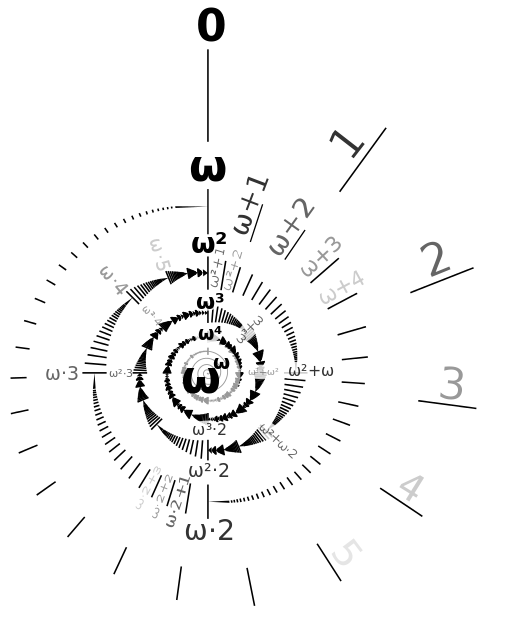
\includegraphics[width=5cm]{ordinal.png}
    \caption{\label{fig:ordinal.png}Ordinaler Zahlenstrahl}
\end{wrapfigure}

\subsection{Ordinalzahlen}
Nun zu der anderen Art von Unendlichkeit, welche ich hier ansprechen moechte.
Auch mit ihr sollten wir vertraut sein.
% Ich bin mir nicht sicher, ob der Ton (den Leser wirzen) fuer solch ein
% Textstueck angemessen ist.
Wir fordern eigentlich nur eine Eigenschaft: die Ordnung muss erhalten
bleiben. Anfänglich sind wir wieder äquivalent zu den natürlichen Zahlen, da
diese bereits eine Wohlordnung haben. Wenn wir nun einen Zahlenstrahl
betrachten, zeichnen wir einen solchen häufig mit $\infty$, umgangssprachlich
"unendlich". %Evtl "Unendlichkeit"? Nicht sicher, was huebscher klingt.
Dieses Zeichen ist nicht Element der natürlichen oder gar reellen
Zahlen, sondern bezeichnet eher ein Element welches größer ist als alle die wir
aufschreiben oder uns vorstellen könnten. Wir definieren uns nun ein Element
$\omega$, das direkt rechts daneben anzuordnen ist, also das erste Element
außerhalb, oder neben, eher nach, dem Zahlenstrahl. Es sollte klar sein dass
es strikt größer ist als alle vorhergehenden Ordinalzahlen, also z.B. alle
Zahlen die auch natürliche Zahlen wären. Die Frage nach $\omega - 1$, also der
Ordinalzahl vor $\omega$, kann nicht beantwortet werden.\\
Intuitiv: es ist nicht
möglich eine feste Zahl direkt vor 'unendlich' zu definieren, denn könnten wir
das, könnten wir diese Zahl so weit erhöhen (um 2) und wären größer als
$\omega$, die ja die größte Zahl sein soll. Allerdings ist zu beachten, dass $1
+ \omega = \omega \neq \omega + 1$. Intuitiv kann man wieder sagen dass eben
kein Element davor, wohl aber ein strikt größeres Element danach gibt, oder
dass man einen Zahlenstrahl wohl auch bei 2 anfangen kann, dieser entsprechend
immernoch gleich lang ist, aber wenn man ein Element nach dem Zahlenstrahl
hinzufügt, muss es immer erst nach dem Zahlenstrahl, strikt hinter allen
anderen Elementen davor, angeordnet sein. Genauso ist $\omega + \omega = \omega
* 2$, oder $\omega * \omega = \omega ^ 2$.


\section{Superturingmaschinen}
% Dieser Satz ist so semigeeignet fuer einen wissenschaftlichen Text ;)
Superturingmaschinen klingen jetzt erstmal total super, und das sind sie auch.
Eigentlich sind es nur Turingmaschinen, außer dass ihre Schritte in
Ordinalzahlen gezählt werden, dass es also Schritte $\omega$, $\omega + 1$,
etc. quasi nach dem Ende der Zeit gibt, wo sie einfach weiterrechnen können.
Dadurch lösen wir das klassische Halteproblem von Turingmaschinen, da wir
einfach schauen können ob unsere Superturingmaschine (die sich ja sonst nicht
unterscheidet) nach dem Ende der Zeit bereits angehalten hat oder eben nicht.
% Um welche Zeit geht es hier? Eine kleine Einfuehrung des Begriffs in einem
% Satz waere fuer mich praktisch.


\subsection{Verhalten bei Grenzen}
% Wieder zu lange Saetze mit zu vielen Kommata
Was natürlich immer passieren kann, ist, dass eine Superturingmaschine nicht
anhält, und ständig weiter eine Zelle mit 1 und anschließend mit 0 beschreibt.
In einem solchen Fall (oder allgemein, wenn sie nicht hält) muss definiert
werden, was anschließend, in Schritt $\omega$ der Zustand sein soll.

Meta: An
diesem Punkt kann auf Supertasks hingewiesen werden, ein Beispiel wäre das
umschalten eines Lichtschalters nach immer halben Zeitintervall zuvor, also
angefangen bei 1s, 0.5s, 0.25s, ... wäre er in Sekunde 2 bei $\omega$
angelangt, allerdings ist bei ständigem umschalten eines Lichtschalters nicht
definiert, in welchem Zustand er anschließend, also nach Sekunde 2, ist.
Außerdem gibt es auch keine eindeutige Antwort, da es gleichzusetzen wäre mit
'Ja, Unendlich ist gerade' oder eben dem Gegenteil davon. Allerdings sollte das
Publikum bereits mit Supertasks im allgemein vertraut sein. Da davon nicht
auszugehen ist, werde ich sie kurz erwähnen, aber dann weitermachen mit:

eine
Turingmaschine die nicht terminiert, in welchem Zustand befindet sie sich zum Zeitpunkt
$\omega$? Weil: es kann einer von vielen sein, gleichzeitig eines von auf die
verschiedensten Weisen beschriebenes Band. Und wieder: egal wie man es festlegt,
% Klingt holprig, mir faellt allerdings nichts sinnvolleres ein.
kann es gut passieren dass Eindeutig ist wie viele und welche Schritte bisher
notwendig gewesen sein müssen, also dass $\omega$ in einem solchen Fall nicht
'nach' dem Zahlenstrahl kommt. Dementsprechend definiert man es folgendermaßen:
Sofern die Turingmaschine hält, ist sie auch nach beliebig vielen weiteren
schritten in ihrem finalen Zustand. Ist dies allerdings nicht passiert, wird
der Schreib-/Lesekopf wieder auf den Anfang gesetzt, sowie die
Superturingmaschine auf ihren Startzustand. Der Einfachheit halber nehmen wir
an, dass
wir nur Nullen (default) und Einsen auf unserem Band haben können. Eine Null
wird nun an Schritt $\omega$ überall dort stehen wo entweder keine Eins
geschrieben wurde, oder nur endlich oft eine Eins geschrieben wurde. Eine Eins
steht hingegen überall dort, wo zu mehr als endlich vielen Zeitpunkten eine
% Wiederum etwas holprig.
Eins stand, bis hin zu von Anfang an (durchgehend). Dementsprechend ist der
Wert einer jeden Zelle entsprechend ihres Limeswertes, und die Turingmaschine
ist wieder auf Anfangszustand, allerdings mit möglicherweise verändertem Band.

\subsection{Fähigkeiten}
Superturingmaschinen können nun natürlich zum einen alles tun, was normale
Turingmaschinen auch können. Außerdem können sie, wie wir eben gesehen haben,
entscheiden ob eine normale Turingmaschine hält oder nicht. Genauso können sie
natürlich neben dem Simulieren von normalen Turingmaschinen auch
Superturingmaschinen simulieren. Was sie allerdings auch entscheiden können
sind $\Sigma_1^1$-Aussagen, also Aussagen der Form 'Es gibt eine Funktion
$\mathbb{N} \rightarrow \mathbb{N}$ so dass ...', sowie $\Pi^1_1$-Aussagen,
also Aussagen der Form 'Für jede Funktion $\mathbb{N} \rightarrow \mathbb{N}$
gilt ...'. 


\subsection{Halteverhalten von STM}





\end{document}
